\documentclass[border=0.5cm]{standalone}
\usepackage{tikz}
\usetikzlibrary{arrows, arrows.meta, tikzmark}

\tikzset{    
    disk/.style={ thick },
    traj/.style={ dotted, -Latex },
    point/.style={ draw, inner sep=1pt, circle, scale=0.4 },
    partition/.style={ right, scale=0.5 }
}

\definecolor{light-gray}{gray}{0.9}

\def\xMin{0}
\def\xMax{9}
\def\yMin{0}
\def\yMax{4}
\def\R{0.75}
\def\gap{0.2}
\def\rowspace{0.1}

\begin{document}
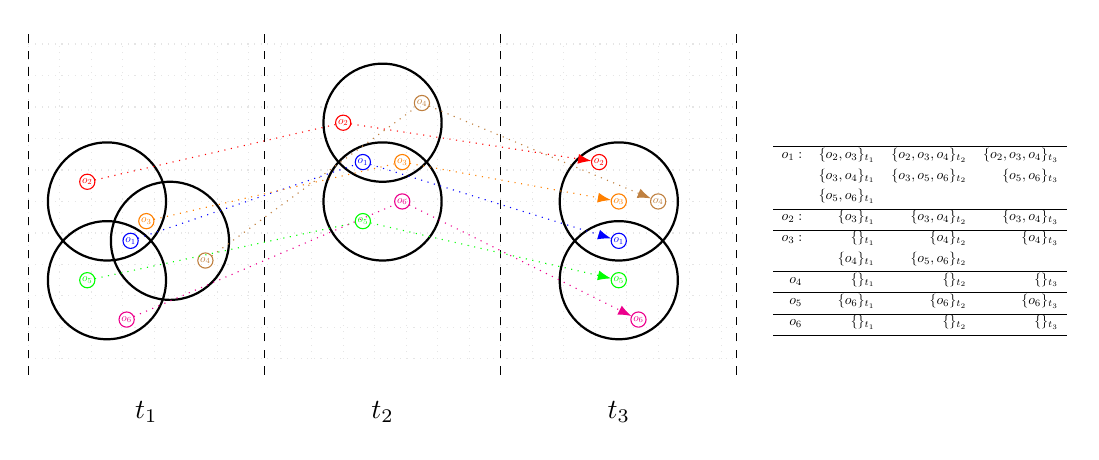
\begin{tikzpicture}
    \draw[color=light-gray, style=dotted, step=0.4] (\xMin,\yMin) grid (\xMax,\yMax);
    \draw[dashed] (0,\yMin-\gap) -- (0,\yMax+\gap);
    \draw[disk] (1,1) circle (\R);
    \draw[disk] (1.8,1.5) circle (\R);
    \draw[disk] (1,2) circle (\R);
    \draw[dashed] (3,\yMin-\gap) -- (3,\yMax+\gap);
    \draw[disk] (4.5,3) circle (\R);
    \draw[disk] (4.5,2) circle (\R);
    \draw[dashed] (6,\yMin-\gap) -- (6,\yMax+\gap);
    \draw[disk] (7.5,2) circle (\R);
    \draw[disk] (7.5,1) circle (\R);
    \draw[dashed] (9,\yMin-\gap) -- (9,\yMax+\gap);
    \node[very thick, below] at (1.5,\yMin-\gap-\gap) {$t_1$};
    \node[very thick, below] at (4.5,\yMin-\gap-\gap) {$t_2$};
    \node[very thick, below] at (7.5,\yMin-\gap-\gap) {$t_3$};

    \node[partition] (partitions) at (\xMax+\gap+\gap, 1.5) {
    \begin{tabular}{r r r r}
        \hline
        $o_1:$  & $\{o_2, o_3\}_{t_1}$  & $\{o_2, o_3, o_4\}_{t_2}$   & $\{o_2, o_3, o_4\}_{t_3}$   \\[\rowspace cm]
                & $\{o_3, o_4\}_{t_1}$  & $\{o_3, o_5, o_6\}_{t_2}$   & $\{o_5, o_6\}_{t_3}$        \\[\rowspace cm]
                & $\{o_5, o_6\}_{t_1}$  &                             &                             \\[\rowspace cm]
        \hline
        $o_2:$  & $ \{o_3\}_{t_1}$      & $\{o_3, o_4\}_{t_2}$        & $\{o_3,o_4\}_{t_3}$         \\[\rowspace cm]
        \hline
        $o_3:$  & $ \{\}_{t_1}$         & $\{o_4\}_{t_2}$             & $\{o_4\}_{t_3}$             \\[\rowspace cm]
                & $ \{o_4\}_{t_1}$      & $\{o_5,o_6\}_{t_2}$         &                             \\[\rowspace cm]
        \hline
        $o_4$   & $ \{\}_{t_1}$         & $\{\}_{t_2}$                & $\{\}_{t_3}$                \\[\rowspace cm]
        \hline
        $o_5$   & $ \{o_6\}_{t_1}$      & $\{o_6\}_{t_2}$             & $\{o_6\}_{t_3}$             \\[\rowspace cm]
        \hline
        $o_6$   & $ \{\}_{t_1}$         & $\{\}_{t_2}$                & $\{\}_{t_3}$                \\[\rowspace cm]
        \hline
    \end{tabular}
    };

    % Trajectories
    \node[point, blue] (o11) at (1.30, 1.50) {$o_1$};
    \node[point, blue] (o12) at (4.25, 2.50) {$o_1$};
    \node[point, blue] (o13) at (7.50, 1.50) {$o_1$};
    %\node[scale=0.1] (oo1) at (\xMax, 2.5) {};
    %\node[partition] (o1) at (\xMax, 2.5) {$o_1$};
    \draw[traj, blue]  (o11)-- (o12) -- (o13);% -- (oo1);

    \node[point, red] (o21) at (0.75, 2.25) {$o_2$};
    \node[point, red] (o22) at (4.00, 3.00) {$o_2$};
    \node[point, red] (o23) at (7.25, 2.50) {$o_2$};
    %\node[scale=0.1] (oo2) at (\xMax, 2) {};
    %\node[partition] (o2) at (\xMax, 2) {$o_2$};
    \draw[traj, red]  (o21)-- (o22) -- (o23);% -- (oo2);

    \node[point, orange] (o31) at (1.50, 1.75) {$o_3$};
    \node[point, orange] (o32) at (4.75, 2.50) {$o_3$};
    \node[point, orange] (o33) at (7.50, 2.00) {$o_3$};
    %\node[scale=0.1] (oo3) at (\xMax, 1.5) {};
    %\node[partition] (o3) at (\xMax, 1.5) {$o_3$};
    \draw[traj, orange]  (o31)-- (o32) -- (o33);% -- (oo3);

    \node[point, brown] (o41) at (2.25, 1.25) {$o_4$};
    \node[point, brown] (o42) at (5.00, 3.25) {$o_4$};
    \node[point, brown] (o43) at (8.00, 2.00) {$o_4$};
    %\node[scale=0.1] (oo4) at (\xMax, 1) {};
    %\node[partition] (o4) at (\xMax, 1) {$o_4$};
    \draw[traj, brown]  (o41)-- (o42) -- (o43);% -- (oo4);

    \node[point, green] (o51) at (0.75, 1.00) {$o_5$};
    \node[point, green] (o52) at (4.25, 1.75) {$o_5$};
    \node[point, green] (o53) at (7.50, 1.00) {$o_5$};
    %\node[scale=0.1] (oo5) at (\xMax, 0.5) {};
    %\node[partition] (o5) at (\xMax, 0.5) {$o_5$};
    \draw[traj, green]  (o51)-- (o52) -- (o53);% -- (oo5);

    \node[point, magenta] (o61) at (1.25, 0.50) {$o_6$};
    \node[point, magenta] (o62) at (4.75, 2.00) {$o_6$};
    \node[point, magenta] (o63) at (7.75, 0.50) {$o_6$};
    %\node[scale=0.1] (oo6) at (\xMax, 0) {};
    %\node[partition] (o6) at (\xMax, 0) {$o_6$};
    \draw[traj, magenta]  (o61)-- (o62) -- (o63);% -- (oo6);

    %%%%%
    %\foreach \i in {\xMin,...,\xMax} { \node[very thin,gray,below,scale=0.5] at (\i,\yMin) {$\i$}; }
    %\foreach \i in {\yMin,...,\yMax} { \node[very thin,gray,left ,scale=0.5] at (\xMin,\i) {$\i$}; }    
    %%%%%
\end{tikzpicture}
\end{document}
